\section{Deep Learning}
\label{sec:dl}

In the field of machine learning, the first models you
are often introduced to are those for regression
and classification that utilize linear
combinations of fixed basis functions.
According to \cite{Bishop:2008aa},
these models possess useful analytical and computational properties,
but their practical applicability is constrained 
since their capacity is limited to linear functions
and they cannot understand the interaction between any two input variables.
This leads to problems such as the \textbf{curse of dimensionality},
where the number of possible interactions between variables grows exponentially
with the number of input variables.
To address large-scale problems, it is essential to adapt the basis functions
to the data, as demonstrated by support vector machines (SVMs).
Alternatively, one can fix the number of basis functions in advance while
allowing them to be adaptive, utilizing parametric forms for the basis
functions with parameter values adjusted during training.

The most successful example of this approach in pattern recognition is the
\textbf{feed-forward neural network},
also known as the multilayer perceptron (MLP).
\begin{figure}[h]
    \centering
    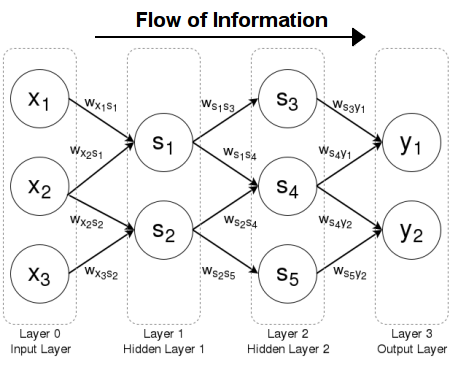
\includegraphics[width=.75\textwidth]{figures/ch3/1.mlp.png}
    \caption{A feed-forward neural network with two hidden layers}
    \vspace{-10px}
    \caption*{\scriptsize{Source: \href{https://brilliant.org/wiki/feedforward-neural-networks/}{Brilliant}}}
    \label{fig:mlp}
\end{figure}

As explained in 
\cite{goodfellow2016deep},
the goal of a feedforward network is to approximate a specific function
\( f^* \). For example, in a classification task,
\( y = f^*(x) \) maps an input \( x \) to a category \( y \).
A feedforward network defines a mapping \( y = f(x; \theta) \) and
learns the parameters \( \theta \) that yield the best approximation
of this function.

These models are called \textbf{feedforward} because information
flows unidirectionally from the input \( x \), through intermediate computations
defining \( f \), and ultimately to the output \( y \), without feedback loops.

The training data directly specifies the output layer's behavior but
not the intermediate layers, which are called \textbf{hidden layers}
because their desired outputs are not provided by the training data.
The learning algorithm must determine how to best utilize these
hidden layers to approximate \( f^* \).
Every layer of the network computes a non-linear transformation of the
previous layer's activations, this way a complex function can be
approximated by composing simpler functions, one for each layer.
Layers are composed of a set of \textbf{units}, where each unit is a node that
computes a non-linear function of the weighted sum of its inputs
and is only connected to units in the previous and the following layer.

In order to train the network and update the weights, MLPs use the
\textbf{backpropagation} technique, which computes the gradient of the
loss function with respect to the weights of the network.
The weights are then updated using an optimization algorithm such as
\textbf{stochastic gradient descent} (SGD)
or one of its adaptive variants like \textbf{Adam},
whose hyperparameters are tuned according to the task during training.

A feedforward network is called a \textbf{deep neural network} if it has
more than one hidden layer, the branch of machine learning that studies
deep neural networks is called \textbf{deep learning}.

They are called networks due to their structure, which involves composing
multiple functions together. Typically, this composition is represented
by a directed acyclic graph. For instance, functions
\( f^{(1)} \), \( f^{(2)} \), and \( f^{(3)} \) might be connected in
a chain to form \( f(x) = f^{(3)}(f^{(2)}(f^{(1)}(x))) \).

Functions \( f^{(1)} \) and \( f^{(2)} \) must
be non linear, otherwise the composition would collapse into a single
linear function. These non-linear functions are
called \textbf{activation functions}.
The last function \( f^{(3)} \) is typically a linear function that maps
the output of the final hidden layer to the output layer.
This is the same as applying a linear model to a transformed
input \( \phi(x) \), where \( \phi \) is a nonlinear transformation.
The question then becomes how to choose the mapping \( \phi \).

The strategy of deep learning is to learn \( \phi \):
in this approach, we use a model
\begin{equation}
y = f(x; \theta, w) = \phi(x; \theta)^\top w
\end{equation}
Here, we have parameters \( \theta \) that are used to learn \( \phi \)
from a broad class of functions, and parameters \( w \) that map \( \phi(x) \)
to the desired output.
This approach allows for greater flexibility:
specifically, by using a broad family of functions
\( \phi(x; \theta) \), the human designer only needs to select the appropriate
general function family rather than finding precisely an exact function.

The \textbf{universal approximation theorem} \cite{HORNIK1989359}
tells us that regardless of what function
we are trying to learn, we know that a feedforward network with enough units
will be able to \emph{represent} this
function, however we are not guaranteed that the training algorithm will be able
to \emph{learn} it.

\subsection{Convolutional Neural Networks}
\label{sec:cnn}

Convolutional Neural Networks (CNNs) are a specialized type of neural network
for processing data that has a known, grid-like topology,
it is particularly effective for image recognition tasks.

The key components of CNNs are:
\begin{itemize}
    \item \textbf{Convolutional layers}: These layers apply a convolution operation
    to the input, passing the result to the next layer.
    The input grid is convolved with a set of filters,
    also known as \textbf{kernels}, which are small windows that move across the input grid
    and apply a convolution operation between the input and the kernel weight
    at each position. The weight of the kernel is learned during training.
    Each convolutional layer applies multiple filters to the input, each producing
    a different \textbf{feature map}.
    \item \textbf{Pooling layers}: These layers downsample the feature maps
    produced by the convolutional layers to reduce the dimensionality of the data.
    This reduces the computational complexity of the network and helps to focus
    on the most important elements of the input.
    \item \textbf{Fully connected} (FC) \textbf{layers}: These layers connect every neuron
    in one layer to every neuron in another layer.
    It is in these layers that the features learned by the convolutional layers
    are used to classify the input image.
\end{itemize}
An example of a CNN classification architecture is shown in Figure \ref{fig:cnn}.

\begin{figure}[h]
    \centering
    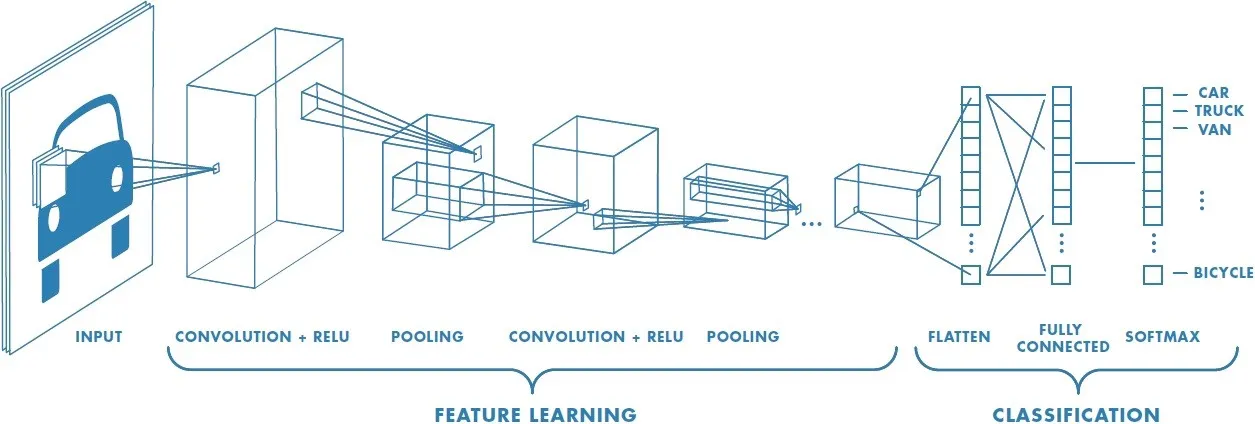
\includegraphics[width=\textwidth]{figures/ch3/8.cnn.png}
    \caption{A typical CNN architecture for classification.}
    \vspace{-10px}
    \caption*{\scriptsize{Source: \href{https://towardsdatascience.com/a-comprehensive-guide-to-convolutional-neural-networks-the-eli5-way-3bd2b1164a53}{Sumit Saha}}}
    \label{fig:cnn}
\end{figure}

CNNs have been shown to achieve state-of-the-art performance on
a variety of computer vision tasks, including image classification,
object detection and image segmentation.
They have also been successfully applied to other types of data,
such as speech recognition and natural language processing.

\section{Reinformcement Learning}
\label{sec:rl}

``\textbf{Reinforcement learning} is learning [...] how
to map situations to actions so
as to maximize a numerical reward signal.
The learner is not told which actions to
take, but instead must discover which actions
yield the most reward by trying them. In
the most interesting and challenging cases, actions may
affect not only the immediate
reward but also the next situation and,
through that, all subsequent rewards.
These two
characteristics, \textbf{trial-and-error search} and \textbf{delayed reward},
are the two most important
distinguishing features of reinforcement learning.'' \cite{sutton1998}

Let's explore the basic concepts of reinforcement learning with
a simple example as described in \cite{zhao2024RLBook}.
Consider a grid world scenario as shown in Figure \ref{fig:rl}
where a robot, referred to as
the \textbf{agent}, moves between cells, occupying one cell at a time.
The white cells are accessible, while the orange cells are forbidden.
The goal is for the agent to reach a target cell.

\begin{figure}[h]
    \centering
    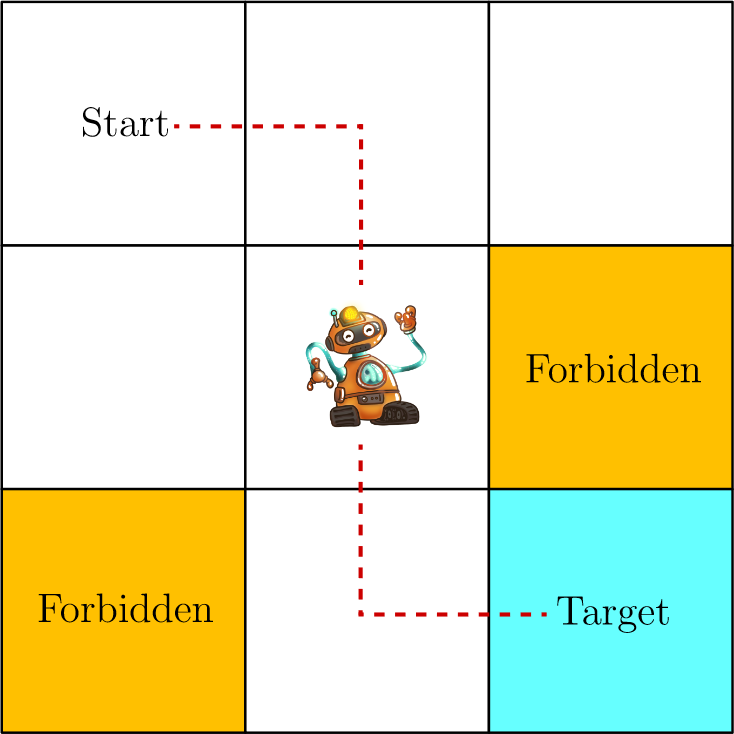
\includegraphics[width=.42\textwidth]{figures/ch3/2.rl.png}
    \caption{A simple reinforcement learning task}
    \vspace{-10px}
    \caption*{\scriptsize{Source: \cite{zhao2024RLBook}}}
    \label{fig:rl}
\end{figure}

To achieve this, the agent needs a \textbf{policy} that guides it to the target
efficiently, avoiding forbidden cells and unnecessary detours.
If the grid layout is known, planning is simple.
However, without prior knowledge, the agent must explore and learn
through trial and error.

The agent's status in the grid is defined by its \textbf{state}
\( s_i \in \mathcal{S} \), which represents its location relative
to the \textbf{environment}.
In the examples with nine cells, the state space is
\( \mathcal{S} = \{s_1, s_2, \ldots, s_9\} \)..

From each state, the agent can perform five \textbf{actions}: move up,
right, down, left or stay put, denoted as \( a_1, a_2, \ldots, a_5 \),
this set of actions is the action space
\( \mathcal{A} = \{a_1, \ldots, a_5\} \).
The available actions can vary by state, for instance,
at \( s_1 \), actions \( a_1 \) (up) and \( a_4 \) (left) would collide
with the grid boundary, so the action space is
\( \mathcal{A}(s_1) = \{a_2, a_3, a_5\} \).

When taking an action, the agent may move from one state to another,
a process known as \textbf{state transition}. For example,
if the agent is at state \( s_1 \) and selects action
\( a_2 \) (moving rightward), it transitions to state
\( s_2 \). This process can be represented as:
\[ s_1 \overset{a_2}{\longrightarrow} s_2 \]
The state transition process is defined for each
state and its associated actions. Mathematically, state transitions
are described by conditional probabilities.
For example, for \( s_1 \) and \( a_2 \),
the conditional probability distribution is:
\[
\begin{aligned}
p(s_1 \mid s_1, a_2) &= 0, \\
p(s_2 \mid s_1, a_2) &= 1, \\
p(s_3 \mid s_1, a_2) &= 0, \\
p(s_4 \mid s_1, a_2) &= 0, \\
p(s_5 \mid s_1, a_2) &= 0,
\end{aligned}
\]
indicating that taking \( a_2 \) at \( s_1 \) guarantees
the agent moves to \( s_2 \), with a probability of one,
and zero probability for other states.

This is a deterministic state transition,
but state transitions can also be stochastic,
requiring conditional probability distributions.
For instance, if random wind gusts affect the grid,
taking action \( a_2 \) at \( s_1 \) might blow the agent to \( s_5 \)
instead of \( s_2 \), resulting in \( p(s_5 \mid s_1, a_2) > 0 \).

A \textbf{policy} is a function that maps states to actions,
indicating the agent's behavior in the environment.
In other words, a policy tells the agent what action to take
at each state.

Mathematically, policies can be described by conditional probabilities.
For example, the policy for \( s_1 \) is:
\[
\begin{aligned}
\pi(a_1 \mid s_1) &= 0, \\
\pi(a_2 \mid s_1) &= 1, \\
\pi(a_3 \mid s_1) &= 0, \\
\pi(a_4 \mid s_1) &= 0, \\
\pi(a_5 \mid s_1) &= 0,
\end{aligned}
\]
indicating that the probability of taking action \( a_2 \) at state \( s_1 \)
is one, and the probabilities of taking other actions are zero.

The above policy is deterministic, but policies may generally be stochastic.
For instance, let's assume that at state \( s_1 \)
the agent may take actions to move either rightward or downward,
each with a probability of 0.5. In this case, the policy for \( s_1 \) is:
\[
\begin{aligned}
\pi(a_1 \mid s_1) &= 0, \\
\pi(a_2 \mid s_1) &= 0.5, \\
\pi(a_3 \mid s_1) &= 0.5, \\
\pi(a_4 \mid s_1) &= 0, \\
\pi(a_5 \mid s_1) &= 0.
\end{aligned}
\]

After executing an action at a state, the agent receives a
reward \( r \) as feedback from the environment.
The \textbf{reward} is a function of the state and action
which predicts immediate reward and is denoted as:
\begin{equation}
R(s_t=s, a_t=a) = \mathbb{E} [r_t | s_t = s, a_t = a]
\end{equation}
and it can be positive, negative, or zero.
Different rewards influence the policy the agent learns.
Generally, a positive reward encourages the agent to take the
corresponding action, while a negative reward discourages it.

However we can't find good policies
by simply selecting actions with the greatest immediate rewards
since they do not consider
long-term outcomes. To determine a good policy, we must consider the total
reward obtained in the long run and
an action with the highest immediate reward may not lead to
the greatest total reward.

A \textbf{trajectory} is a state-action-reward chain.
For example, the agent in our example may follow this trajectory:
\[ s_1 \xrightarrow{a_2, r=0} s_2 \xrightarrow{a_3, r=0} s_5 \xrightarrow{a_3, r=0} s_8 \xrightarrow{a_2, r=1} s_9. \]
The \textbf{return} of this trajectory is the sum of all rewards collected along it,
in the example above:
\[\text{return} = 0+0+0+1=1\]
Returns, also called total rewards or cumulative rewards,
are used to evaluate policies.
Returns can also be defined for infinitely long trajectories, which may diverge.
Therefore, we introduce the concept of \textbf{discounted return} for infinitely
long trajectories. The discounted return is the sum of the rewards from $t$ to $T$ (final step):
\begin{equation}
G_t \doteq R_{t+1} + \gamma R_{t+2} + \gamma^2 R_{t+3} + \ldots = \sum_{k=0}^{\infty} \gamma^k R_{t+k+1}
\end{equation}
where \( \gamma \in [0, 1] \) is the \textbf{discount factor}.
If \( \gamma \) is close to 0, the agent emphasizes near-future rewards,
resulting in a short-sighted policy. If \( \gamma \) is close to 1,
the agent emphasizes far-future rewards.

When $T$ is finite, we call the task episodic and each sequence
up to the \textbf{terminal state} is an \textbf{episode}. Otherwise, we refer
to \textbf{continuing tasks}.

The \textbf{Markov Decision Processes} (MDPs),
a general framework for describing stochastic dynamical systems,
allows us to formally presents these concepts.
The \textbf{Markov property} refers to the \textbf{memoryless} property of a stochastic process. Mathematically, it means that
\begin{equation}
\begin{aligned}
p(s_{t+1} \mid s_t, a_t, s_{t-1}, a_{t-1}, \ldots, s_0, a_0) &= p(s_{t+1} \mid s_t, a_t), \\
p(r_{t+1} \mid s_t, a_t, s_{t-1}, a_{t-1}, \ldots, s_0, a_0) &= p(r_{t+1} \mid s_t, a_t),
\end{aligned}
\end{equation}
where \( t \) represents the current time step and \( t + 1 \) represents the next time step.
This indicates that the next state or reward depends only on the current
state and action and is independent of the previous ones.

\vspace{3cm}

An MDP is defined by a tuple \( \langle \mathcal{S}, \mathcal{A}, P, R, \gamma \rangle \),
let us break down the components:
\begin{itemize}
    \item \( \mathcal{S} \): finite set of Markov states $s$
    \item \( \mathcal{A} \): finite set of actions $a$
    \item \( P \): state transition model for each action,
    a probability matrix that specifies $$p(s_t+1 = s'|s_t=s, a_t=a)$$
    \item \( R \): reward function
    $$ R(s_t=s, a_t=a) = \mathbb{E} [r_t | s_t = s, a_t = a] $$
    \item \( \gamma \): discount factor $0 \leq \gamma \leq 1$
\end{itemize}

When the policy in a MDP is fixed, it reduces to a \textbf{Markov Process} (MP),
this transformation simplifies the MDP by eliminating the decision-making aspect. 
A Markov process is referred to as a \textbf{Markov Chain} if it operates in discrete
time and the number of states is either finite or countable.

\begin{figure}[h]
    \centering
    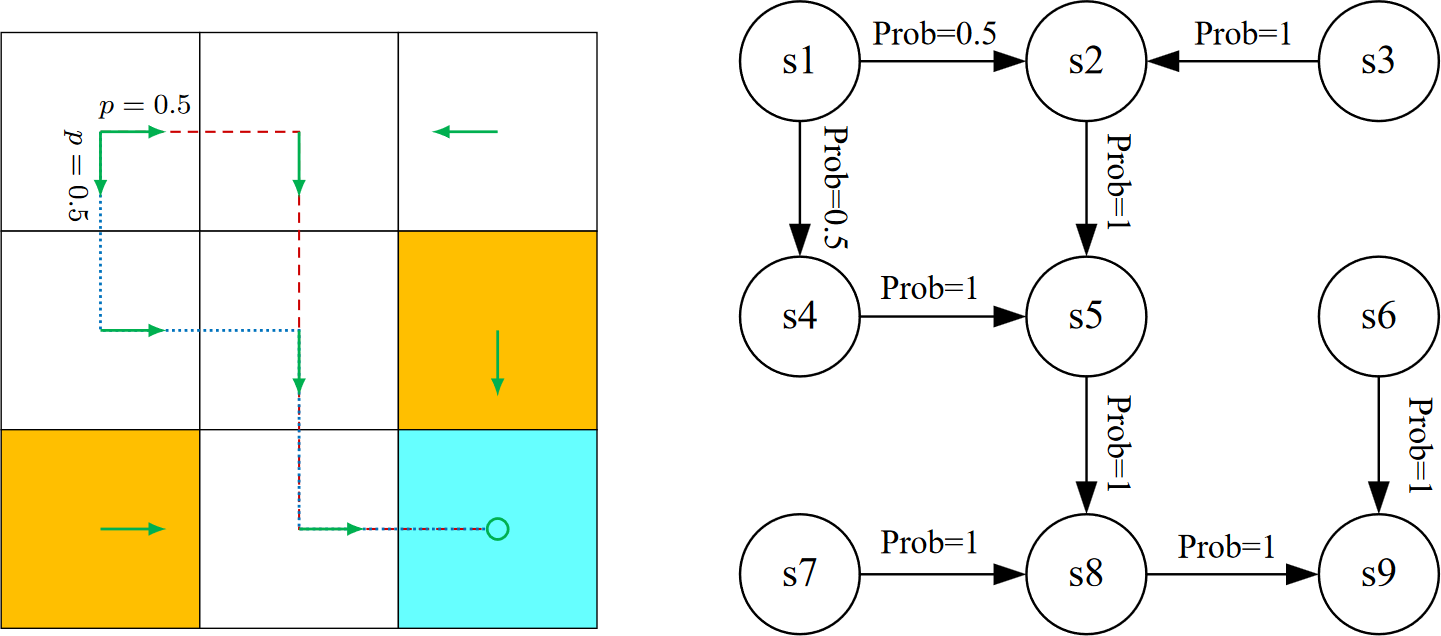
\includegraphics[width=.75\textwidth]{figures/ch3/3.mdp.png}
    \caption{The example grid as a Markov Process graph, where the nodes
    represent the states and the edges represent the state transitions.}
    \vspace{-10px}
    \caption*{\scriptsize{Source: \cite{zhao2024RLBook}}}
    \label{fig:mdp}
\end{figure}


\subsection{Reinforcement Learning Algorithms}
\label{sec:rlalg}

In \cite{openaiPartKinds}, the landscape of algorithms in modern reinforcement
learning is explored.

The algorithms used in reinforcement learning almost always rely on
\textbf{value functions}.
The \textbf{value} is the expected return if the agent starts in
that state or state-action pair and then follows a specific policy indefinitely.

\vspace{5cm}

There are four primary value functions to consider:

\begin{itemize}
    \item \textbf{On-Policy Value Function, \( V^{\pi}(s) \)}: This function
    represents the expected return if the agent starts in state \( s \)
    and acts according to the policy \( \pi \):
    \begin{equation}
    V^{\pi}(s) = \mathbb{E}_{\tau \sim \pi} \left[ R(\tau) \mid s_0 = s \right]
    \end{equation}
    \item \textbf{On-Policy Action-Value Function, \( Q^{\pi}(s,a) \)}:
    This function gives the expected return if the agent starts in state \( s \),
    takes an arbitrary action \( a \), and then always follows the policy \( \pi \):
    \begin{equation}
    Q^{\pi}(s,a) = \mathbb{E}_{\tau \sim \pi} \left[ R(\tau) \mid s_0 = s, a_0 = a \right]
    \end{equation}
    \item \textbf{Optimal Value Function, \( V^*(s) \):} This function provides
    the expected return if the agent starts in state \( s \) and follows the
    optimal policy for the environment:
    \begin{equation}
    V^*(s) = \max_{\pi} \mathbb{E}_{\tau \sim \pi} \left[ R(\tau) \mid s_0 = s \right]
    \end{equation}
    \item \textbf{Optimal Action-Value Function, \( Q^*(s,a) \):} This function
    represents the expected return if the agent starts in state \( s \),
    takes an arbitrary action \( a \), and then follows the optimal policy for the environment:
    \begin{equation}
    Q^*(s,a) = \max_{\pi} \mathbb{E}_{\tau \sim \pi} \left[ R(\tau) \mid s_0 = s, a_0 = a \right]
    \end{equation}
\end{itemize}

Figure \ref{fig:mdp}
presents a partial taxonomy of the modern reinforcement learning algorithms.
One key distinction is whether the agent utilizes (or learns) a model of
the environment. A model, in this context, refers to a function that predicts
state transitions and rewards.

\begin{figure}[h]
    \centering
    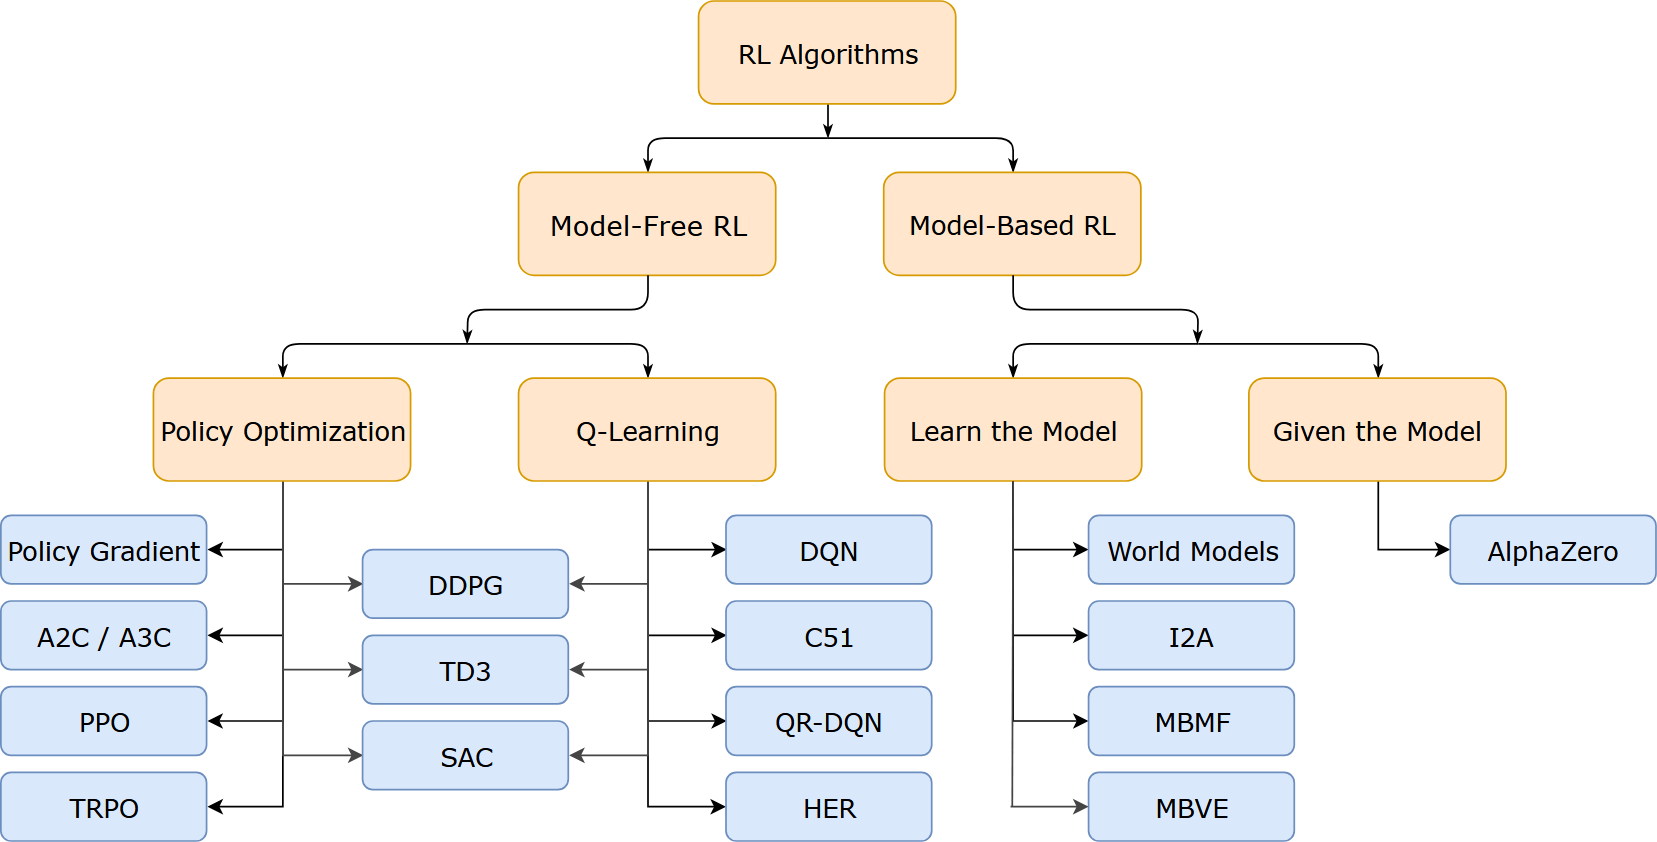
\includegraphics[width=.8\textwidth]{figures/ch3/4.rlalg.png}
    \caption{Partial taxonomy of algorithms in modern RL.}
    \vspace{-10px}
    \caption*{\scriptsize{Source: \cite{openaiPartKinds}}}
    \label{fig:mdp}
\end{figure}

The primary advantage of having a model is that it enables the agent
to plan by predicting future states and rewards.
However, the major drawback is that an accurate model of the environment
is often unavailable to the agent.
Algorithms which use a model are known as \textbf{model-based} methods,
while those that do not are referred to as \textbf{model-free} methods.
Our focus will be on the latter.

Model-free methods can be categorized into two main approaches
for representing and training agents:
\begin{itemize}
    \item \textbf{Policy Optimization:} explicitly represents a policy
    as \( \pi_{\theta}(a \mid s) \) and optimizes the parameters \( \theta \)
    either directly via gradient ascent on the performance objective
    \( J(\pi_{\theta}) \) or indirectly by maximizing local approximations
    of \( J(\pi_{\theta}) \).
    Typically, this optimization is performed \textbf{on-policy},
    meaning that each update uses data collected while the agent is acting
    according to the most recent version of the policy.

    \item \textbf{Q-Learning:} involves learning an approximator
    \( Q_{\theta}(s,a) \) for the optimal action-value function \( Q^*(s,a) \).
    Unlike policy optimization, Q-learning is generally performed \textbf{off-policy},
    allowing updates to use data collected at any time during training,
    irrespective of the agent's policy at the time of data collection.
    The corresponding policy is derived from the relationship between
    \( Q^* \) and \( \pi^* \), where the actions taken by the Q-learning
    agent are determined by
    \begin{equation}
    a(s) = \arg \max_a Q_{\theta}(s,a)
    \end{equation}
    An example of a Q-learning algorithm is Deep Q-Network (\textbf{DQN})
    \cite{dqn},
    which uses a deep neural network to approximate the optimal action-value
    function in environments with large state spaces,
    and its variants such as Double DQN (\textbf{DDQN})
    \cite{ddqn} and
    Dueling Double DQN (\textbf{D3QN}) \cite{d3qn}.

\end{itemize}

There are also hybrid approaches that combine elements
of both policy optimization and Q-learning.
In this spectrum of algorithms we can find 
\textbf{actor-critic methods}, which consist of two components:
an \textbf{actor} that makes actions and a \textbf{critic} that evaluates them.
An example of an actor-critic algorithm is Twin-Delayed DDPG (\textbf{TD3})
\cite{td3}.

If samples are collected during training the reinforcement learning is
considered \textbf{online}, otherwise,
if the training set is fixed, it is \textbf{offline}.

\section{Generative Adversarial Networks}
\label{sec:gan}

\textbf{Generative Adversarial Networks} (GANs) is a framework
for estimating generative models via an adversarial process,
initially introduced by \cite{goodfellow2014}.
This framework involves training two models:
a \textbf{generative} model \( G \), which captures the data
distribution, and a \textbf{discriminative} model \( D \),
which predicts samples as either originating from the true
data distribution or the generative model.
The training objective for \( G \) is to maximize
the likelihood of \( D \) making incorrect classifications.
This adversarial process can be conceptualized as a minimax two-player game.
In the theoretical space of arbitrary functions \( G \) and \( D \),
a unique solution exists where \( G \) accurately
recovers the training data distribution and \( D \) outputs $\frac{1}{2}$
for all inputs (in other words, it reaches maximum uncertainty).
When \( G \) and \( D \) are defined by multilayer perceptrons,
the entire system can be trained using backpropagation.

To learn the generator's distribution \( p_G \)
over data \( x \), we define a prior \( p_z(z) \) on input noise variables
$z \in \Omega_Z$, called \textbf{latent distribution},
and represent a mapping to the data space as
\( G(z; \theta_g) \), where \( G: \Omega_Z \rightarrow \Omega_X \)
is a differentiable function parameterized by \( \theta_g \).
Additionally, we define a second network
\( D(x; \theta_d) \) that outputs a single scalar,
representing the probability that \( x \) originated
from the true data distribution $p_x$ rather than from \( p_G \).
The discriminative model \( D \) is trained to maximize
the probability of correctly labeling both the training
examples and the samples generated by \( G \).
Simultaneously, the generative model \( G \) is trained to minimize
\( \log(1 - D(G(z))) \).

Formally, \( D \) and \( G \) engage in the following
two-player minimax game with the value function \( V(G, D) \):
\begin{equation}
\min_G \max_D V(D, G) = \mathbb{E}_{x \sim p_X(x)}[\log D(x)] + \mathbb{E}_{z \sim p_Z(z)}[\log (1 - D(G(z)))].
\end{equation}

We can see a graphical representation of the GAN framework in Figure \ref{fig:gan}.
\begin{figure}[h]
    \centering
    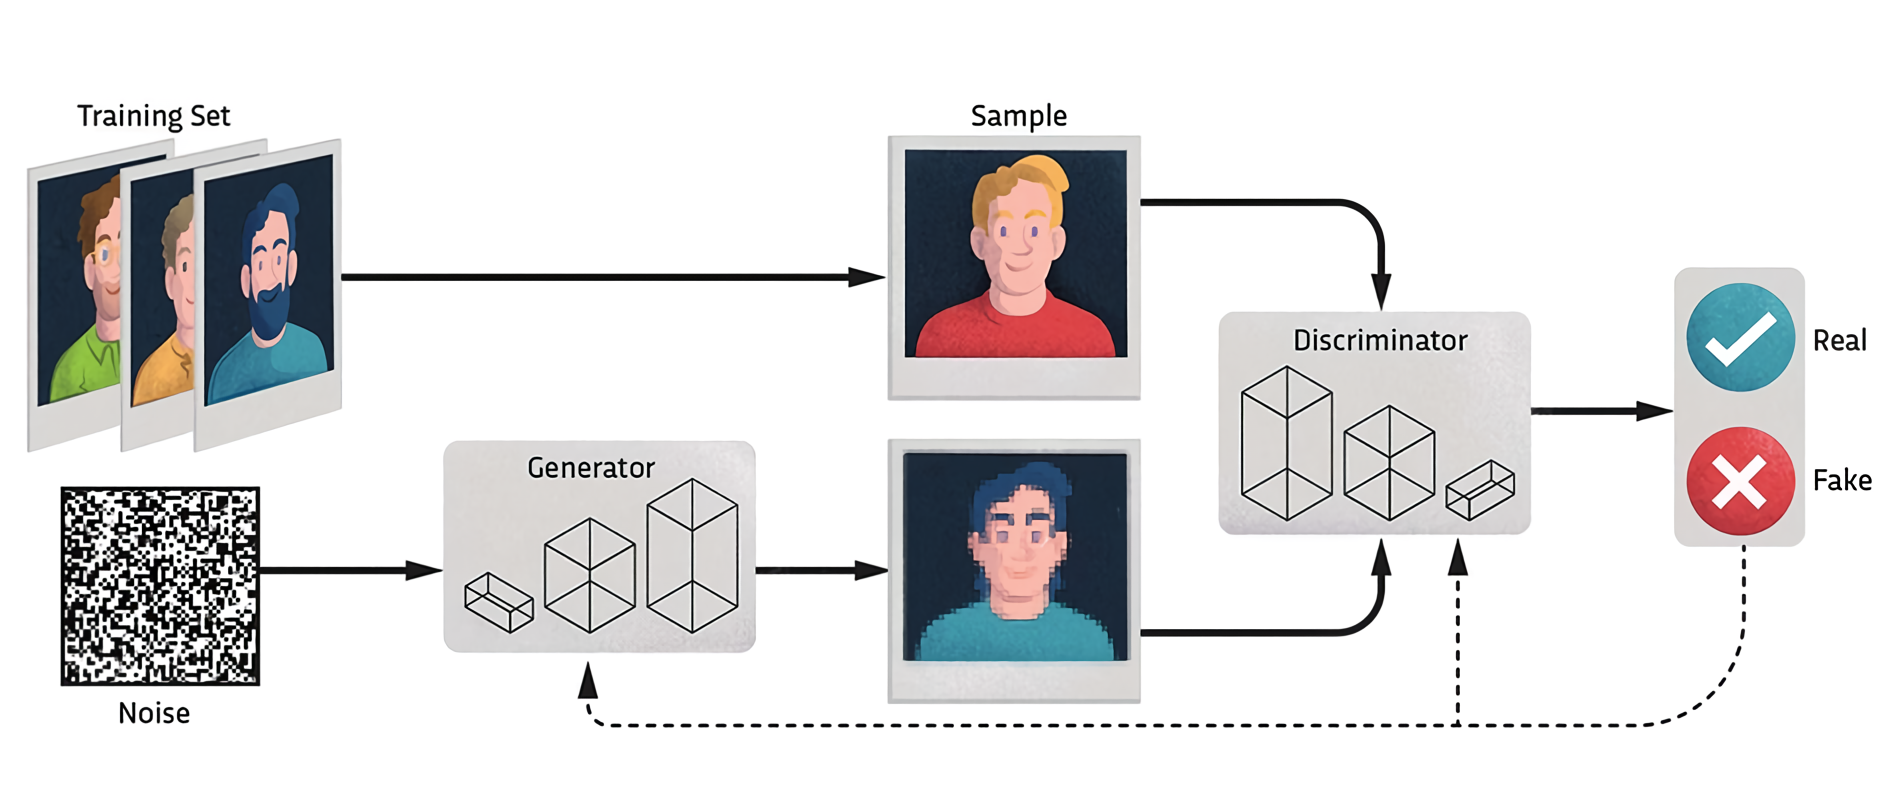
\includegraphics[width=\textwidth]{figures/ch3/5.gan.png}
    \caption{GAN framework applied to human faces generation task}
    \vspace{-10px}
    \caption*{\scriptsize{Source: \href{https://www.linkedin.com/pulse/exploring-fascinating-realm-generative-adversarial-networks-kaurav/}{Yashwant Singh Kaurav}}}
    \label{fig:gan}
\end{figure}

\subsection{Bidirectional GANs}
\label{sec:bigan}

Generative Adversarial Networks (GANs) have the potential to be used
for unsupervised learning of rich feature representations across various
data distributions. However, an obvious issue arises because
the GAN framework inherently lacks an inverse mapping from generated data
back to the latent representation.
This limitation means that while the generator can map latent samples
to generated data, there is no mechanism to map data back to the latent space.

To address this issue, \cite{donahue2017} introduced a novel framework
called Bidirectional Generative Adversarial Networks (BiGAN).
The BiGAN framework, whose architecture is illustrated
in Figure \ref{fig:bigan}, enhances the standard GAN model
(as introduced by \cite{goodfellow2014}) by incorporating an \textbf{encoder}.
This encoder, denoted as \( E: \Omega_X \rightarrow \Omega_Z \),
maps data \( x \) to latent representations
\( z \), complementing the generator \( G \).

\begin{figure}[h]
    \centering
    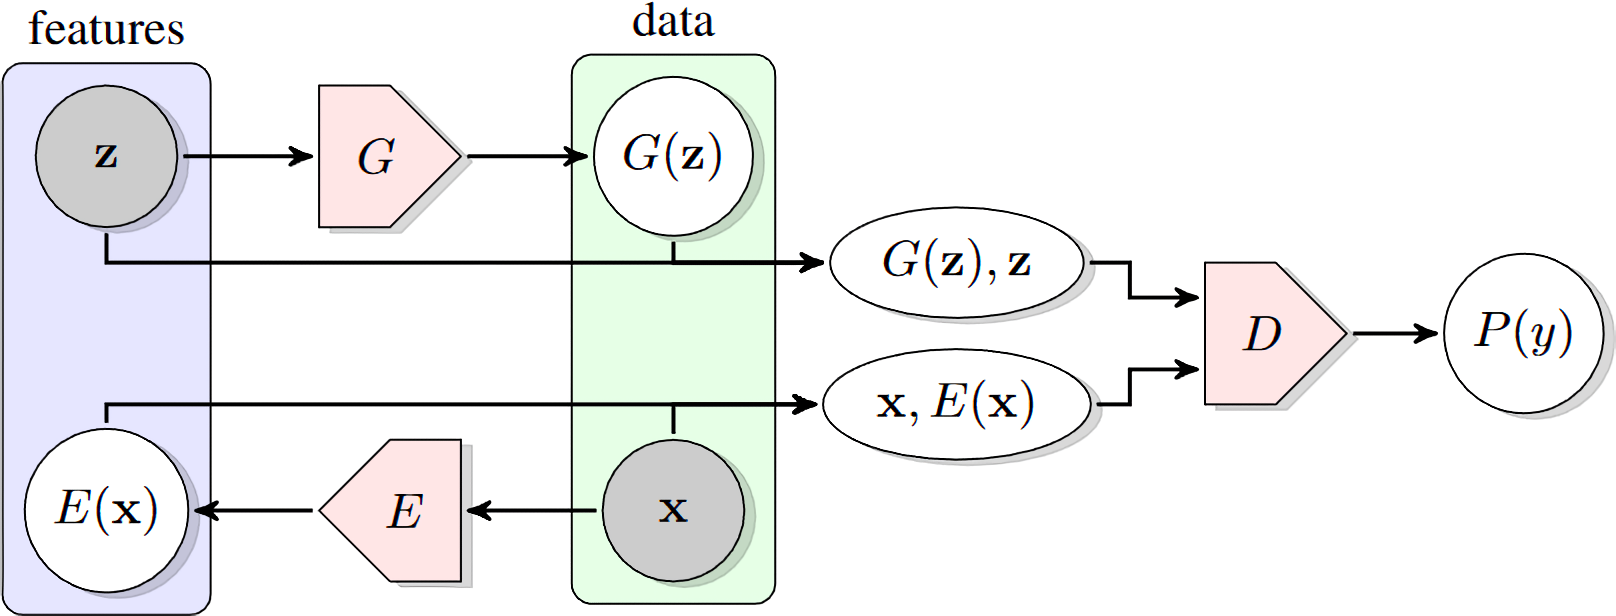
\includegraphics[width=\textwidth]{figures/ch3/6.bigan.png}
    \caption{BiGAN architecture with generator, discriminator, and encoder.}
    \vspace{-10px}
    \caption*{\scriptsize{Source: \cite{donahue2017}}}
    \label{fig:bigan}
\end{figure}

In BiGAN, the discriminator \( D \) operates not only in the data space
(distinguishing between \( x \) and \( G(z) \)) but also jointly in the
data and latent spaces. Specifically, the discriminator evaluates pairs
of data and their corresponding latent representations, distinguishing
between real \( (x, E(x)) \) and generated \( (G(z), z) \).
Here, the latent component is either an encoder output \( E(x) \) 
or a generator input \( z \).

An essential aspect of BiGAN is that the encoder \( E \) is designed
to learn an inverse mapping of the generator \( G \).
Despite the encoder and generator not directly interacting, since
\( E(G(z)) \) is not explicitly computed and the generator does not use
\( E(x) \), the framework ensures that the encoder effectively inverts
the generator's mapping.

The training objective for BiGANs is formulated as a minimax problem involving the generator \( G \), the encoder \( E \), and the discriminator \( D \). This objective can be written as:
\[
\min_{G, E} \max_{D} V(D, E, G)
\]
where the value function \( V(D, E, G) \) is defined as:
\begin{equation}
V(D, E, G) := \mathbb{E}_{x \sim p_X} [ \underset{\log D(x,\, E(x)) }{\underbrace{\mathbb{E}_{z \sim p_E(\cdot | x)} \left[ \log D(x, z) \right]}}  ] +
\mathbb{E}_{z \sim p_Z} [ \underset{\log(1 - D(G(z),\, z))}{\underbrace{\mathbb{E}_{x \sim p_G(\cdot | z)} \left[ \log(1 - D(x, z)) \right]}} ].
\end{equation}
In simpler terms, this objective consists of two components:
\begin{enumerate}
    \item The expectation over the data distribution \( p_X \)
    and the encoder's latent space distribution \( p_E(\cdot | x) \),
    which aims to maximize \( \log D(x, E(x)) \).
    \item The expectation over the prior distribution \( p_Z \)
    and the generator's data distribution \( p_G(\cdot | z) \),
    which aims to maximize \( \log(1 - D(G(z), z)) \).
\end{enumerate}

The optimization of this minimax objective is performed
using an alternating gradient-based approach, similar to the method
introduced by \cite{goodfellow2014} for GANs.

\subsection{Bidirectional Conditional GANs}
\label{sec:bicogan}

Conditional GAN (cGAN) (\cite{mirza2014})
is a variant of standard GANs designed to enable the
conditional generation of data samples based on both latent variables
(intrinsic factors) and known auxiliary information (extrinsic factors)
such as class labels or associated data from other modalities.
However, cGANs fails to achieve several key properties:

\begin{enumerate}
    \item The ability to disentangle intrinsic and extrinsic
    factors during the generation process.
    \item The ability to separate the components of extrinsic
    factors from each other, ensuring that the inclusion of one
    factor minimally impacts the others.
\end{enumerate}

\cite{jaiswal2018} introduced the Bidirectional Conditional GAN (BiCoGAN).
BiCoGAN enhances the cGAN framework by simultaneously training an encoder
along with the generator and discriminator.
This encoder learns inverse mappings of data samples to both intrinsic
and extrinsic factors, thereby overcoming deficiencies in prior approaches.
In Figure \ref{fig:bicogan}, we present the architecture of BiCoGAN.

\begin{figure}[h]
    \centering
    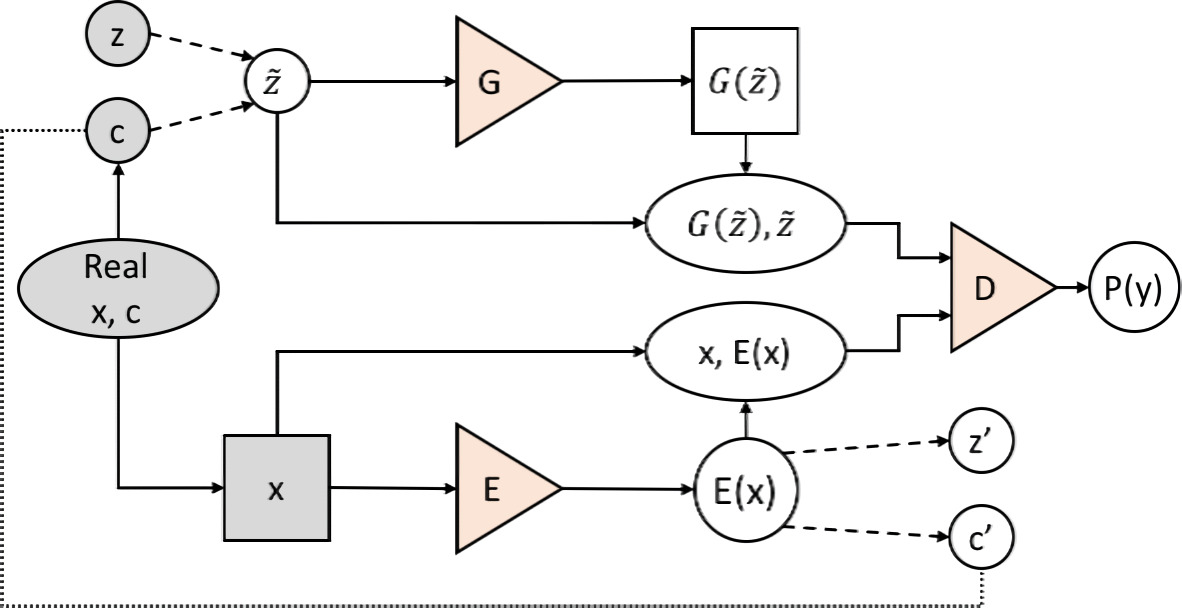
\includegraphics[width=.8\textwidth]{figures/ch3/7.bicogan.jpeg}
    \caption{BiCoGAN architecture with generator, discriminator, and encoder.}
    \vspace{-10px}
    \caption*{\scriptsize{Source: \cite{jaiswal2018}}}
    \label{fig:bicogan}
\end{figure}

In the BiCoGAN framework, the generator
\( G(\tilde{z}; \theta_G) \) learns a mapping from the distribution
\( p_{\tilde{Z}} \), where \( \tilde{z} = [z, c] \), to \( p_G \),
with the goal of making \( p_G \) approximate \( p_X \). Concurrently,
the encoder \( E(x; \theta_E) \) learns a mapping from \( p_X \) to \( p_E \),
aiming to make \( p_E \) approximate \( p_{\tilde{Z}} \). The discriminator
\( D \) evaluates real or fake decisions using pairs
\( (\tilde{z}, G(\tilde{z}); \theta_D) \) and \( (E(x), x; \theta_D) \).

The encoder in BiCoGAN must effectively learn the inverse mapping from data
\( x \) to latent variables \( z \) and conditions \( c \),
just as the generator must incorporate both to produce data samples
that can deceive the discriminator. This requirement follows from the
invertibility under the optimality theorem of BiGANs.
However, achieving this optimality is challenging in practice,
especially when the prior vector contains structured or complex information.
While intrinsic factors \( z \) are sampled from a simple latent distribution,
extrinsic factors \( c \), such as class labels or object attributes,
have specialized and complex distributions that are more difficult to model.

To address this challenge, we introduce the
\textbf{extrinsic factor loss} (EFL) as a mechanism to guide BiCoGANs
in better encoding extrinsic factors. During training, the condition
\( c \) associated with each real data sample is known and can be used to
improve the learning of inverse mappings from \( x \) to \( c \).
The specific form of EFL depends on the nature of \( c \) and the dataset
or domain in question.

The BiCoGAN value function can be expressed as:
\begin{equation}
\begin{aligned}
V(D, G, E) &:= \mathbb{E}_{x \sim p_X(x)} [\log D(E(x), x)]\\
&\quad + \gamma \, \mathbb{E}_{(x, c) \sim p_X(x, c)} [\text{EFL}(c, E_c(x))] \\
&\quad +\mathbb{E}_{z \sim p_{\tilde{Z}} (\tilde{z})} [\log (1 - D(\tilde{z}, G(\tilde{z})))]
\end{aligned}
\end{equation}
where \( \gamma \) is the \textbf{extrinsic factor loss weight} (EFLW),
defined as:
\[
\gamma = \min(\alpha e^{\rho t}, \phi)
\]
Here, \( \alpha \) is the initial value of \( \gamma \), \( \phi \)
is its maximum value, \( \rho \) controls the rate of exponential increase,
and \( t \) indicates the number of epochs the model has been trained.

\subsection{Wasserstein GANs}
\label{sec:wgan}

In a Generative Adversarial Network (GAN),
the interaction between the generator \( G \) and the discriminator
\( D \) is formalized as a minimax optimization problem:
\begin{equation}
\min_G \max_D \, \mathbb{E}_{x \sim p_X}[\log(D(x))] + \mathbb{E}_{\tilde{x} \sim p_G}[\log(1 - D(\tilde{x}))],
\end{equation}
where \( p_X \) represents the real data distribution,
and \( p_G \) represents the model distribution implicitly defined by
\(\tilde{x} = G(z)\), with \( z \sim p(z) \). If the discriminator
is optimally trained before each update of the generator's parameters,
minimizing this objective corresponds to minimizing the
Jensen-Shannon divergence between \( p_X \) and \( p_G \).
However, this often leads to vanishing gradients as the discriminator saturates.

An alternative approach involves using the \textbf{Earth-Mover distance}
(also known as the Wasserstein-1 distance),
\( W(q, p) \), which measures the minimum cost of transporting mass
to transform distribution \( q \) into distribution \( p \).
Under mild assumptions, \( W(q, p) \) is continuous and differentiable
almost everywhere.

The \textbf{Wasserstein GAN} (WGAN) (\cite{gulrajani2017}) modifies the value
function using the Kantorovich-Rubinstein duality:
\[
\min_G \max_{D \in \mathcal{D}} \, \mathbb{E}_{x \sim p_X}[D(x)] - \mathbb{E}_{\tilde{x} \sim p_G}[D(\tilde{x})],
\]
where \( \mathcal{D} \) is the set of 1-Lipschitz functions,
and \( p_G \) is again the model distribution defined by \(\tilde{x} = G(z)\),
with \( z \sim p(z) \). When the discriminator (referred to as the \textbf{critic}
in this context) is optimal, minimizing the value function with respect
to the generator's parameters minimizes \( W(p_X, p_G) \).

The WGAN value function leads to a critic function with more well-behaved
gradients with respect to its input, facilitating easier optimization
of the generator. Empirically, the WGAN value function has been observed
to correlate better with sample quality compared to the traditional GAN value
function.

To enforce the Lipschitz constraint on the critic, a \textbf{gradient penalty}
is used.
A differentiable function is 1-Lipschitz if its gradients have a norm of at most
1 everywhere. Therefore, the gradient norm of the critic's output with respect
to its input is directly constrained. The new objective is:
\[
L = \mathbb{E}_{\tilde{x} \sim p_G}[D(\tilde{x})] - \mathbb{E}_{x \sim p_X}[D(x)] + \lambda \, \mathbb{E}_{\hat{x} \sim p_{\hat{X}}}[(\|\nabla_{\hat{x}} D(\hat{x})\|_2 - 1)^2],
\]
where the first two terms represent the original critic loss and the
third term is the gradient penalty.

\section{Causal Inference}

The \textbf{causal inference} is a discipline that studies the relationships
of cause-and-effect between variables. Specifically, it is concerned with inferring
the causes of an observed phenomenon,
distinguishing between \textbf{correlation} and \textbf{causality}.
We are going to explore the basic concepts of causal inference
as described in \cite{Neal_2020a}.

\subsection{Correlation does not imply Causation}
\label{sec:correlation}

Consider the following scenario: you come across some data showing a correlation
between wearing shoes to bed and waking up with a headache.
It appears that most people who wear shoes to bed tend to wake up
with a headache, while those who don’t wear shoes to bed typically
do not wake up with a headache.
It is common for people to interpret such data,
where there is an \textbf{association},
as indicating that wearing shoes
to bed causes headaches. This is especially true if they are
seeking a reason to avoid wearing shoes to bed.

We can explain the association between wearing shoes to bed and waking
up with a headache without implying that one causes the other.
Both events are actually caused by a \textbf{common factor}:
drinking the night before. This relationship is depicted
in Figure \ref{fig:confounding}.

\begin{figure}[h]
    \centering
    \begin{subfigure}{.5\textwidth}
      \centering
      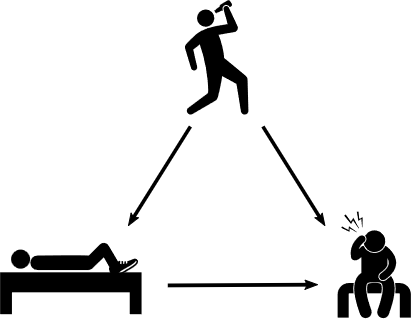
\includegraphics[width=.65\linewidth]{figures/ch3/9.conf.png}
    \end{subfigure}%
    \begin{subfigure}{.5\textwidth}
      \centering
      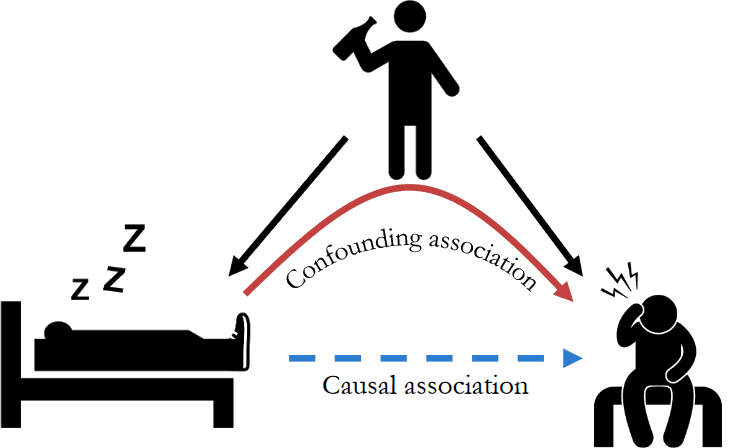
\includegraphics[width=.75\linewidth]{figures/ch3/10.confcol.png}
    \end{subfigure}
    \caption{A confounding variable causes both wearing shoes to bed and waking up with a headache.}
    \vspace{-10px}
    \caption*{\scriptsize{Source: \cite{Neal_2020a}}}
    \label{fig:confounding}
\end{figure}

This kind of variable is often referred to as a \textbf{confounder} and
we refer to this type of association as a \textbf{confounding association}
since the observed relationship is influenced by a confounder.


\subsection{The Flow of Association and Causation in Graphs}
\label{sec:flow}

In the context of modeling associations between variables,
we utilize Directed Acyclic Graphs (DAGs).
The following assumptions are pertinent to this modeling approach:

\begin{itemize}
    \item \textbf{Minimality Assumption}: composed of:
    \begin{itemize}
        \item \textbf{Local Markov Assumption} (LMA):
        Each node is conditionally independent of its
        non-descendants given its parents.
        \item \textbf{Dependency of Adjacent Nodes}: Nodes that
        are adjacent in the DAG are dependent.
    \end{itemize}
    \item \textbf{Bayesian Network Factorization} (BNF): The joint probability
    distribution can be factorized as
    \begin{equation}
        P(x_1, \ldots, x_n) = \prod_i P(x_i \mid \text{pa}_i)
    \end{equation}
    where \( \text{pa}_i \) denotes the parents of node \( x_i \).
    If \( P \) factorizes \( G \), then \( P \) is Markovian with
    respect to \( G \), in fact the Local Markov Assumption is valid
    if and only if the Bayesian Network Factorization is also valid.
    \item \textbf{Causal Edges Assumption}: In a DAG, every parent is
    a direct cause of all its children.
\end{itemize}

But what is a \textbf{cause}? A variable \( X \) is said to be a cause
of a variable \( Y \) if \( X \) can change in response to changes in \( Y \).

In Figure \ref{fig:assumptions}, we can see how implementing each one
of these assumptions leads to having different relationships
between the variables in the graph.

\begin{figure}[h]
    \centering
    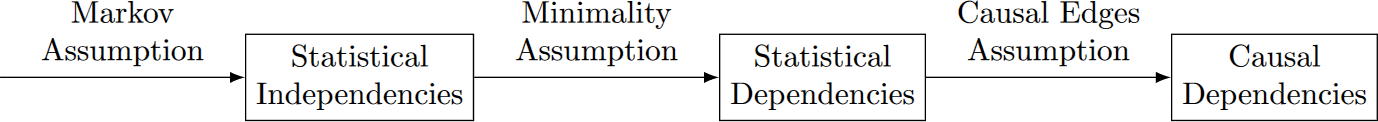
\includegraphics[width=\textwidth]{figures/ch3/15.assumptions.png}
    \caption{Different relationships between variables in a graph based on the assumptions.}
    \vspace{-10px}
    \caption*{\scriptsize{Source: \cite{Neal_2020a}}}
    \label{fig:assumptions}
\end{figure}

This brings us to the core of this section: understanding the flow
of association and causation in DAGs. We can comprehend this flow
in general DAGs by analyzing the minimal building blocks of graphs.

By \textbf{flow of association}, we mean whether any two nodes in
a graph are associated or not associated. In other words, whether two nodes are
(statistically) dependent or (statistically) independent.
Additionally, we will explore whether two nodes are conditionally
independent or not.

Consider a graph consisting of just two unconnected nodes,
as depicted in Figure \ref{fig:unconnected_nodes}.

\begin{figure}[h]
    \centering
    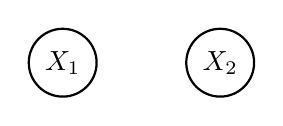
\begin{tikzpicture}[->,shorten >=1pt,auto,node distance=2cm, 
        thick,main node/.style={circle,fill=white,draw,font=\sffamily\bfseries}]

      \node[main node] (1) {$X_1$};
      \node[main node] (2) [right of=1] {$X_2$};

    \end{tikzpicture}
    \caption{Graph with two unassociated nodes.}
    \label{fig:unconnected_nodes}
\end{figure}

These nodes are not associated simply because there is no edge between them.
This can be demonstrated by considering the factorization of \( P(x_1, x_2) \)
given by the Bayesian Network Factorization:
\[
P(x_1, x_2) = P(x_1) P(x_2)
\]
This factorization immediately proves that the two nodes
\( X_1 \) and \( X_2 \) are unassociated (independent)
in this basic structure. The key assumption here is that \( P \)
is Markov with respect to the graph in Figure \ref{fig:unconnected_nodes}.

In contrast, if there is an edge between the two nodes
(as in Figure \ref{fig:connected_nodes}),
then the nodes are associated.
\begin{figure}[h]
    \centering
    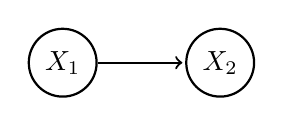
\begin{tikzpicture}[->,shorten >=1pt,auto,node distance=2cm, 
        thick,main node/.style={circle,fill=white,draw,font=\sffamily\bfseries}]

      \node[main node] (1) {$X_1$};
      \node[main node] (2) [right of=1] {$X_2$};

      \path[every node/.style={font=\sffamily\small}]
        (1) edge node {} (2);
    \end{tikzpicture}
    \caption{Graph with two nodes \(X_1\) and \(X_2\) with an arrow from \(X_1\) to \(X_2\), indicating that \(X_1\) is a cause of \(X_2\).}
    \label{fig:connected_nodes}
\end{figure}
The assumption used
here is the causal edges assumption, which indicates that
\( X_1 \) is a cause of \( X_2 \). Since \( X_1 \) is a
cause of \( X_2 \), \( X_2 \) must be able to change
in response to changes in \( X_1 \), establishing their
association. Generally, any time two nodes are adjacent
in a causal graph, they are associated.

Let's now consider more the building blocks of DAGs
as shown in Figure
\ref{fig:building}, where we have a
\textbf{chain}, a \textbf{fork} and an \textbf{immorality}.

\begin{figure}[h]
    \centering
    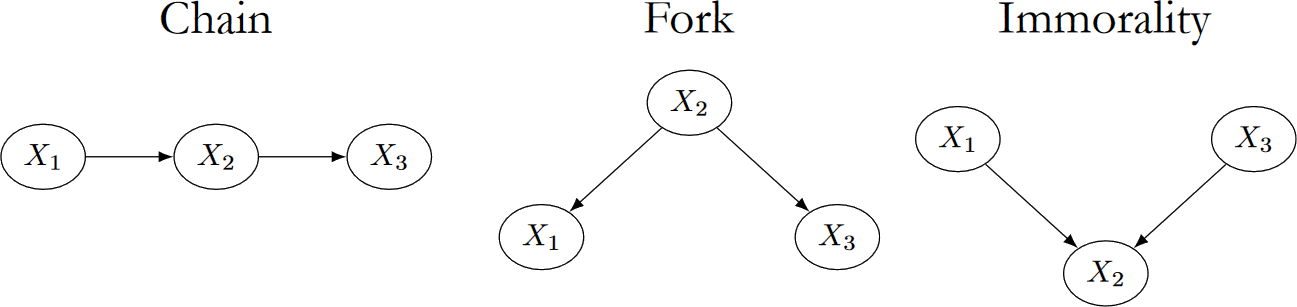
\includegraphics[width=\linewidth]{figures/ch3/16.building.png}
    \caption{Building blocks of DAGs: chain, fork, and immorality.}
    \vspace{-10px}
    \caption*{\scriptsize{Source: \cite{Neal_2020a}}}
    \label{fig:building}
\end{figure}

Chains and forks share the same set of dependencies.
In both structures, \(X_1\) and \(X_2\) are dependent,
and \(X_2\) and \(X_3\) are dependent for the same reason discussed
for the graph in Figure \ref{fig:connected_nodes}.
Adjacent nodes are always dependent when we make the causal edges assumption.
But does association flow from \(X_1\) to \(X_3\) through
\(X_2\) in chains and forks?

In chain graphs, \(X_1\) and \(X_3\) are usually dependent simply because
\(X_1\) causes changes in \(X_2\), which then causes changes in \(X_3\).
In a fork graph, \(X_1\) and \(X_3\) are also usually dependent
because the value that \(X_2\) takes on determines both the value that
\(X_1\) takes on and the value that \(X_3\) takes on. In other words,
\(X_1\) and \(X_3\) are associated through their shared common cause.
However, while in chains the association between \(X_1\) and \(X_3\)
is a causal one, in forks it is not.

Chains and forks also share the same set of independencies.
When we condition on \(X_2\) in both graphs,
it blocks the flow of association from \(X_1\) to \(X_3\).
This is due to the local Markov assumption; each variable can locally
depend only on its parents. Therefore, when we condition
on \(X_2\) (the parent of \(X_3\) in both graphs), \(X_3\)
becomes independent of \(X_1\) (and vice versa).

We refer to this independence as an instance of a blocked path.
These blocked paths are illustrated in Figure \ref{fig:blocked_paths}.

\begin{figure}[h]
    \centering
    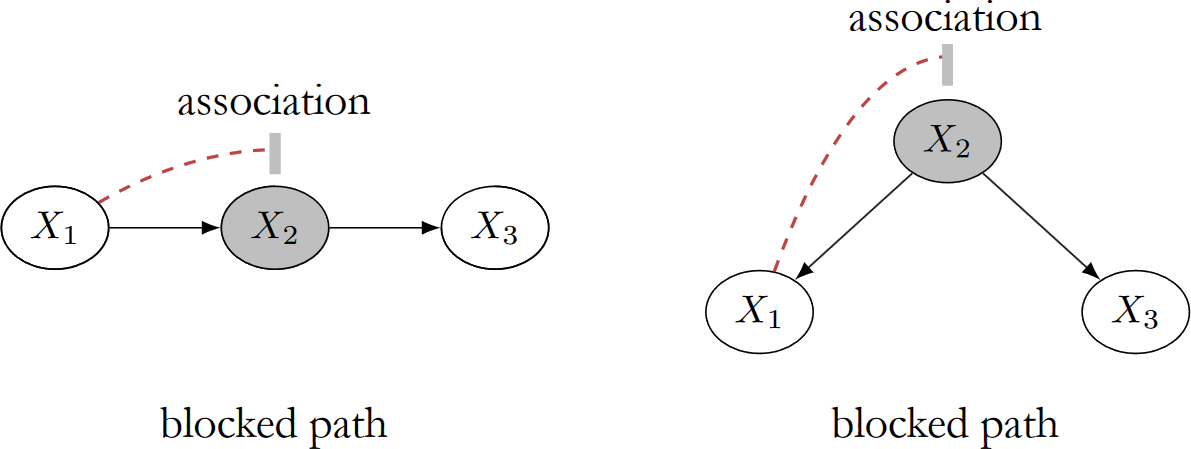
\includegraphics[width=.65\linewidth]{figures/ch3/18.blocked.png}
    \caption{Blocked paths in chain and fork graphs.}
    \vspace{-10px}
    \caption*{\scriptsize{Source: \cite{Neal_2020a}}}
    \label{fig:blocked_paths}
\end{figure}

In contrast to chains and forks, in an immorality, \(X_1 \perp X_3\).
We observe that conditioning on a collider can turn a blocked path
into an unblocked path. The parents \(X_1\) and \(X_3\)
are not associated in the general population, but when we condition
on their shared child \(X_2\) taking on a specific value,
they become associated. Conditioning on the collider \(X_2\)
allows association to flow along the path
\(X_1 \rightarrow X_2 \leftarrow X_3\), despite the fact that it
does not when we do not condition on \(X_2\).
In Figure \ref{fig:immorality}, we can see the immorality with
the blocked path and the unblocked path.

\begin{figure}[h]
    \centering
    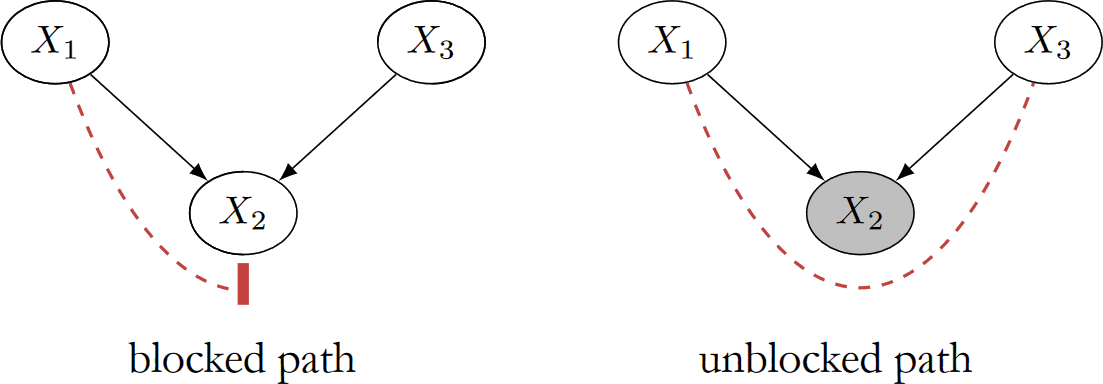
\includegraphics[width=.65\linewidth]{figures/ch3/19.immorality.png}
    \caption{Immorality with a blocked path and an unblocked path.}
    \vspace{-10px}
    \caption*{\scriptsize{Source: \cite{Neal_2020a}}}
    \label{fig:immorality}
\end{figure}

Conditioning on \textbf{descendants of a collider} also induces
association between the parents of the collider.
The intuition is that if we learn something about a collider's descendant,
we usually also learn something about the collider itself because there
is a direct causal path from the collider to its descendants.
In Figure \ref{fig:descendants}, we can see a conditioning
on a descendant of a collider.

\begin{figure}[h]
    \centering
    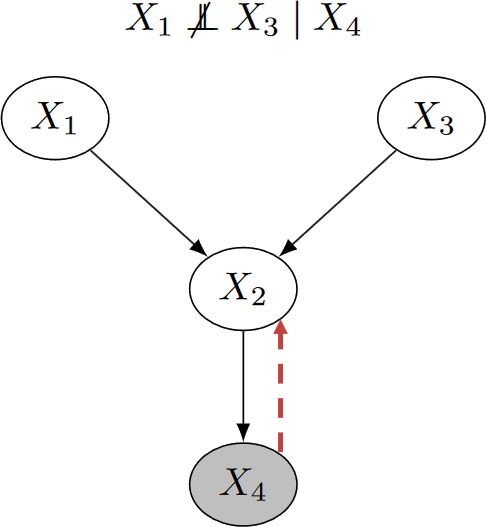
\includegraphics[width=.25\linewidth]{figures/ch3/20.descendant.png}
    \caption{Conditioning on a descendant of a collider.}
    \vspace{-10px}
    \caption*{\scriptsize{Source: \cite{Neal_2020a}}}
    \label{fig:descendants}
\end{figure}

Now let's formally codify the concept of a \textbf{blocked path}:
a path between nodes \( X \) and \( Y \) is \textbf{blocked} by a
(potentially empty) conditioning set \( Z \) if either of the following
is true:
\begin{enumerate}
    \item Along the path, there is a chain
    \(\cdots \rightarrow W \rightarrow \cdots\) or a fork
    \(\cdots \leftarrow W \rightarrow \cdots\),
    where \( W \) is conditioned on (\( W \in Z \)).
    \item There is a \textbf{collider} \( W \) on the path
    that is not conditioned on (\( W \notin Z \)) and none
    of its descendants are conditioned on (\( de(W) \nsubseteq Z \)).
\end{enumerate}

An \textbf{unblocked path} is simply a path that is not blocked.
The graphical intuition to have in mind is that \textbf{association} flows along
unblocked paths and does not flow along blocked paths.

Now, we are ready to introduce
\textbf{d-separation}: two (sets of) nodes \( X \) and \( Y \) are
\textbf{d-separated} by a set of nodes \( Z \) if all of the paths
between (any node in) \( X \) and (any node in) \( Y \) are blocked by \( Z \)
(\cite{pearl1988}).

Otherwise, they are \textbf{d-connected}.


\subsection{Potential Outcomes and the Fundamental Problem of Causal Inference}
\label{sec:potential_outcomes}

The central issue driving the need for causal inference is that
correlation does not imply causation. If these two concepts were equivalent,
causal inference would be easy.
This raises the critical question: how can we determine when one
event causes another and, therefore, infer causality?

To address this, we introduce the concept of \textbf{potential outcomes}.
Suppose, as shown in Figure \ref{fig:potential_outcomes},
you have a headache, and you know that taking a pill would alleviate
the headache, whereas not taking the pill would result in the
headache persisting. In this scenario, you can infer a causal effect
of the pill on the headache. However, if not taking the pill
also resulted in the headache disappearing, you would conclude
that there is no causal effect.
This is the intuition behind potential outcomes.

\begin{figure}[h]
    \centering
    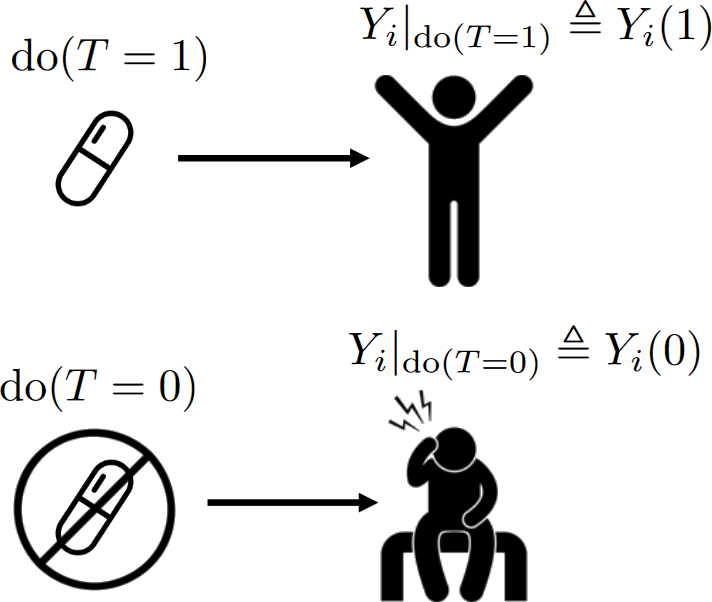
\includegraphics[width=.75\textwidth]{figures/ch3/11.potential.png}
    \caption{Potential outcomes for a causal effect.}
    \vspace{-10px}
    \caption*{\scriptsize{Source: \cite{Neal_2020a}}}
    \label{fig:potential_outcomes}
\end{figure}

Let's define some notation:
\begin{itemize}
    \item \( T \): Observed treatment
    \item \( Y \): Observed outcome
    \item \( i \): Denotes a specific unit or individual
    \item \( Y_i|_{\text{do}(T=1)} \triangleq Y_i(1) \): Potential outcome under treatment
    \item \( Y_i|_{\text{do}(T=0)} \triangleq Y_i(0) \): Potential outcome under no treatment
    \item \( \text{\textbf{Causal Effect}} = Y_i(1) - Y_i(0) \)
\end{itemize}


To account for individual differences, we measure the
\textbf{Average Treatment Effect} (ATE), given by:
\begin{equation}
\mathbb{E}[Y(1)] - \mathbb{E}[Y(0)].
\end{equation}

A fundamental problem in causal inference is the challenge
of distinguishing between the observational distribution
\( P(Y|T=t) \) and the interventional distribution \( P(Y|\text{do}(T=t)) \).
These distributions are generally not equal; if they were, correlation
would indeed imply causation. The intervention \( T=t \) on a population
is denoted by the do-operator, which allows us to measure the causal
effect from the interventional distribution \( P(Y|\text{do}(T=t)) \).

However, we often cannot intervene on the entire population
and can only access the observational distribution.
The distinction between these distributions is illustrated
in Figure \ref{fig:dooperator}.
Intervening with \( \text{do}(T=0) \) (\textbf{factual}) usually
precludes access to \( \text{do}(T=1) \) (\textbf{counterfactual}).

\begin{figure}[h]
    \centering
    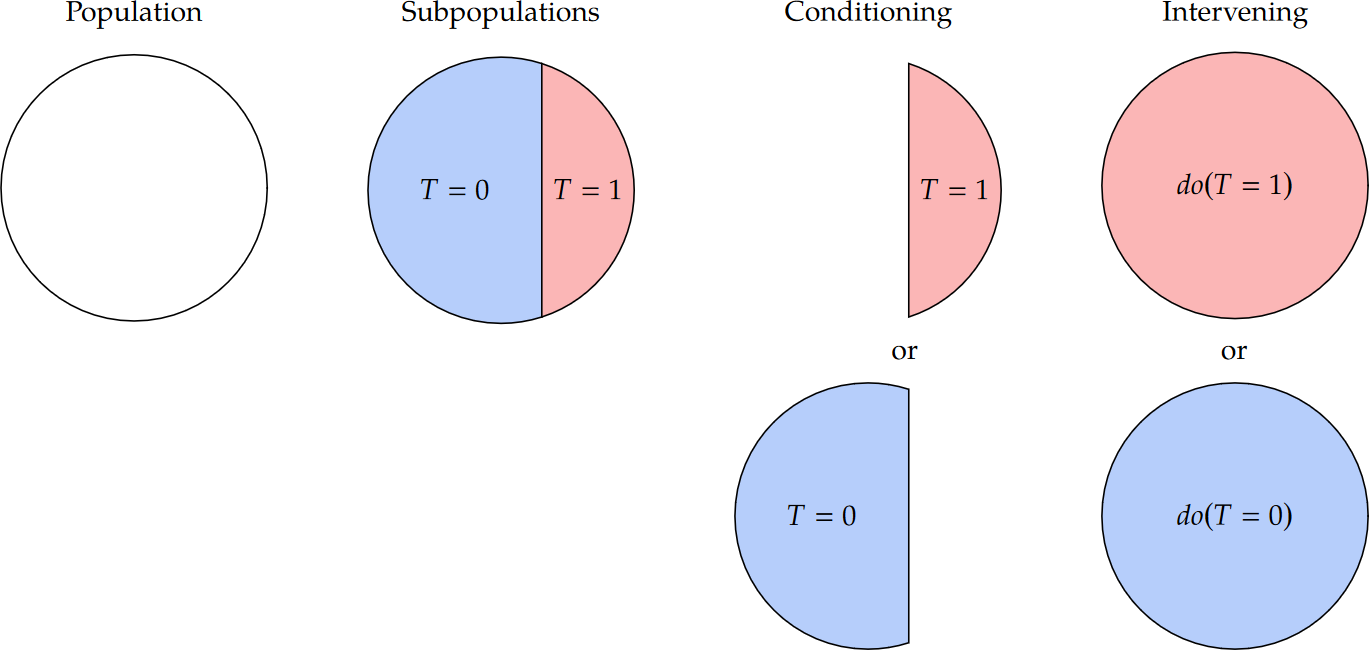
\includegraphics[width=\textwidth]{figures/ch3/12.dooperator.png}
    \caption{The difference between observational and interventional distributions.}
    \vspace{-10px}
    \caption*{\scriptsize{Source: \cite{Neal_2020a}}}
    \label{fig:dooperator}
\end{figure}

One approach to address this issue is
through a \textbf{Randomized Controlled Trial} (RCT). In an RCT, participants
are randomly assigned to treatment or control groups, ensuring that
\( (Y(1), Y(0)) \perp\!\!\!\perp T \), under the assumption of exchangeability.
\textbf{Exchangeability} means that the treatment groups are comparable in the
sense that if they were swapped, the new treatment group would exhibit
the same outcomes as the original treatment group, and the new control
group would exhibit the same outcomes as the original control group.
The randomization process ensures that, as we can see in Figure \ref{fig:rct},
the causal association between the treatment and the outcome is identifiable
since there is no confounding due to a missing connection between the
treatment and the cause.

\begin{figure}[h]
    \centering
    \begin{subfigure}{.5\textwidth}
      \centering
      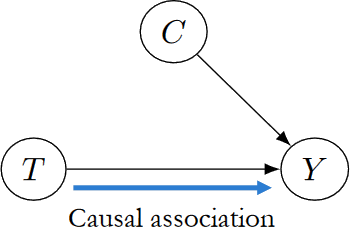
\includegraphics[width=.8\linewidth]{figures/ch3/13.rct1.png}
    \end{subfigure}%
    \begin{subfigure}{.5\textwidth}
      \centering
      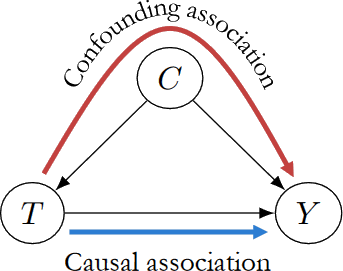
\includegraphics[width=.8\linewidth]{figures/ch3/14.rct2.png}
    \end{subfigure}
    \caption{Randomized Controlled Trial (RCT) design vs. Observational Study.}
    \vspace{-10px}
    \caption*{\scriptsize{Source: \cite{Neal_2020a}}}
    \label{fig:rct}
\end{figure}

However, it is not always feasible to randomize treatment due to several reasons:
\begin{itemize}
    \item \textbf{Ethical reasons}: For instance, it would be unethical
    to randomize people to smoke in order to measure the effect on lung cancer.
    \item \textbf{Infeasibility}: It is impractical to randomize
    countries into different economic systems
    (e.g. communist vs. capitalist) to measure the effect on GDP.
    \item \textbf{Impossibility}: Certain changes, such as altering a
    person's DNA at birth to measure the effect on breast cancer,
    are simply not possible.
\end{itemize}
We must then find a way to estimate causal effects from observational data.

\subsection{Causal Models and Identification}
\label{sec:causal_models}

\textbf{Identification} is the process of moving from a \textbf{causal estimand}
to a \textbf{statistical estimand}. As we have seen in \ref{sec:potential_outcomes},
conditioning on \( T = t \) means that we are restricting our focus to the subset
of the population who received treatment \( t \). In contrast, an \textbf{intervention}
(denoted with the \textbf{do-operator}) involves taking the entire population and
giving everyone treatment \( t \).

\textbf{Interventional distributions} such as \( P(Y \mid do(T = t)) \)
are conceptually quite different from the \textbf{observational distribution} \( P(Y) \)
since the latter do not include the do-operator.
Because of this, we can observe data from them without conducting any experiments.
This is why we call data from \( P(Y, T, X) \) \textbf{observational data}.
If we can reduce an expression \( Q \) with do in it (an interventional expression)
to one without do in it (an observational expression), then \( Q \) is said to be
\textbf{identifiable}. We will refer to an estimand as a
\textbf{causal estimand} when it contains a do-operator,
and as a \textbf{statistical estimand} when it does not contain a do-operator.

Before describing a very important assumption, we must specify what
a \textbf{causal mechanism} is,
we will refer to the causal mechanism that generates \( X_i \)
as the conditional distribution of \( X_i \) given all of
its causes: \( P(x_i \mid \text{pa}_i) \).

To achieve many causal identification results, the main assumption we will
make is that interventions are local:
intervening on a variable \( X_i \) only changes the causal mechanism for \( X_i \).
In this sense, the causal mechanisms are \textbf{modular}.

\textbf{Assumption of Modularity / Independent Mechanisms / Invariance}:\\
If we intervene on a set of nodes \( S \subseteq [n] \)\footnote{We use \( [n] \) to refer to the set \(\{1, 2, \ldots, n\}\).}, setting them to constants, then for all \( i \), we have the following:
\begin{enumerate}
    \item If \( i \notin S \), then \( P(x_i \mid \text{pa}_i) \) remains unchanged.
    \item If \( i \in S \), then \( P(x_i \mid \text{pa}_i) = 1 \) if \( x_i \)
    is the value that \( X_i \) was set to by the intervention; otherwise,
    \( P(x_i \mid \text{pa}_i) = 0 \).
\end{enumerate}

The modularity assumption allows us to encode many different interventional
distributions in a single graph. For example, it could be the case that
\( P(Y) \), \( P(Y \mid do(T = t)) \), \( P(Y \mid do(T = t')) \), and
\( P(Y \mid do(T_2 = t_2)) \) are all completely different distributions that
share almost nothing. If this were the case, each of these distributions would
need its own graph. However, by assuming modularity, we can encode them all
with the same graph that we use to encode the joint \( P(Y, T, T_2, \ldots) \),
and we can know that all of the factors (except the ones that are intervened on)
are shared across these graphs.

The \textbf{causal graph} for interventional distributions,
as shown in an example in Figure \ref{fig:intervention},
is simply the same graph used for the observational joint distribution,
but with all of the edges to the intervened node(s) removed.
This is because the probability for the intervened factor has been set to 1,
allowing us to ignore that factor.

\begin{figure}[h]
    \centering
    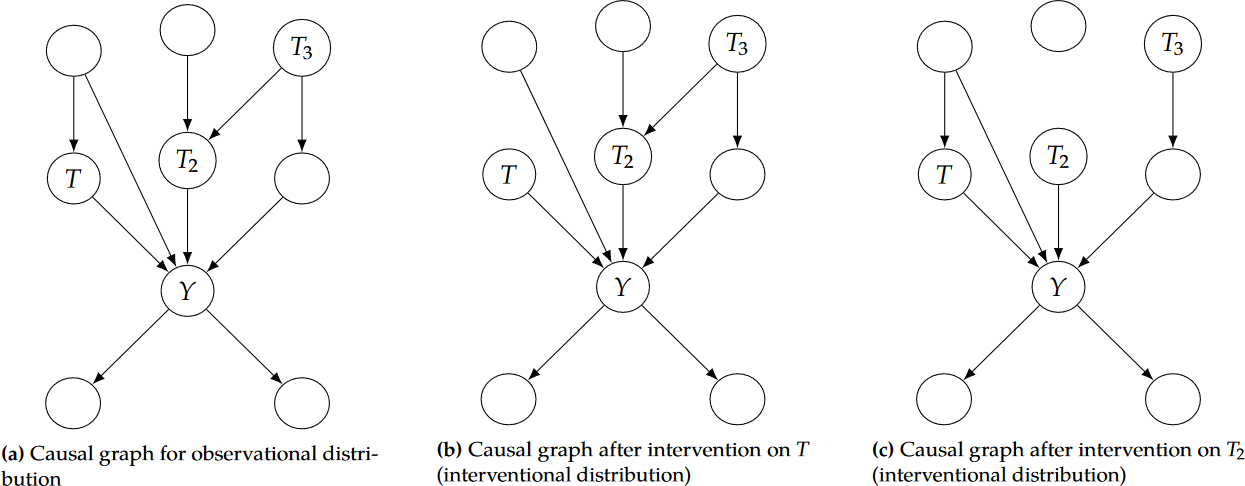
\includegraphics[width=\textwidth]{figures/ch3/21.intervention.png}
    \caption{Intervention as edge deletion in causal graphs.}
    \vspace{-10px}
    \caption*{\scriptsize{Source: \cite{Neal_2020a}}}
    \label{fig:intervention}
\end{figure}

Recall from subsection \ref{sec:flow}, that \textbf{causal association}
flows from \( T \) to \( Y \) along directed paths,
while \textbf{non-causal association} can flow along other
paths from \( T \) to \( Y \) unless they are blocked by either
a non-collider that is conditioned on or a collider that is not
conditioned on. These non-directed unblocked paths from
\( T \) to \( Y \) are known as \textbf{backdoor paths}
because they have an edge that goes in the ``backdoor'' of the \( T \) node.
By conditioning on certain variables, we can block these paths and
identify causal quantities like \( P(Y \mid \text{do}(T = t)) \).

Our goal is to transform the causal estimand
\( P(y \mid \textbf{do}(T = t)) \) into a statistical estimand
that relies only on the observational distribution.
We start by assuming we have a set of variables \( W \) that satisfy
the \textbf{backdoor criterion}:\\
A set of variables \( W \) satisfies the backdoor criterion relative to \( T \) and \( Y \) if the following are true:
\begin{enumerate}
    \item \( W \) blocks all backdoor paths from \( T \) to \( Y \).
    \item \( W \) does not contain any descendants of \( T \).
\end{enumerate}

When \( W \) satisfies the backdoor criterion,
it becomes a \textbf{sufficient adjustment set}.
Additionally, we must ensure \textbf{positivity},
which means that all subgroups of the data with different
covariates have some probability of receiving any value of treatment.
Formally, we define \textbf{positivity} for binary treatment as follows:\\
For all values of covariates \( x \) present in the population of
interest (i.e., \( x \) such that \( P(X = x) > 0 \)),
\[
0 < P(T = 1 \mid X = x) < 1
\]

\textbf{Backdoor Adjustment}: Given the modularity assumption,
that \( W \) satisfies the backdoor criterion, and positivity, 
we can identify the causal effect of \( T \) on \( Y \):
\begin{equation}
P(y \mid \textbf{do}(T = t)) = \sum_{w} P(y \mid T = t, W = w) P(w)
\end{equation}

This theorem connects to \textbf{d-separation}.
We can use the backdoor adjustment if \( W \)
\textbf{d-separates} \( T \) from \( Y \) in the manipulated graph.
Recall that isolating the causal association means
identifying it. We achieve this if \( T \) is d-separated from
\( Y \) in the manipulated graph or if \( Y \)
is d-separated from \( T \) in the manipulated graph,
conditional on \( W \).
In Figure \ref{fig:backdoor}, we can see how the backdoor paths
that are blocked by conditioning on \( W \) allow
us to identify the causal effect of \( T \) on \( Y \).

\begin{figure}[H]
    \centering
    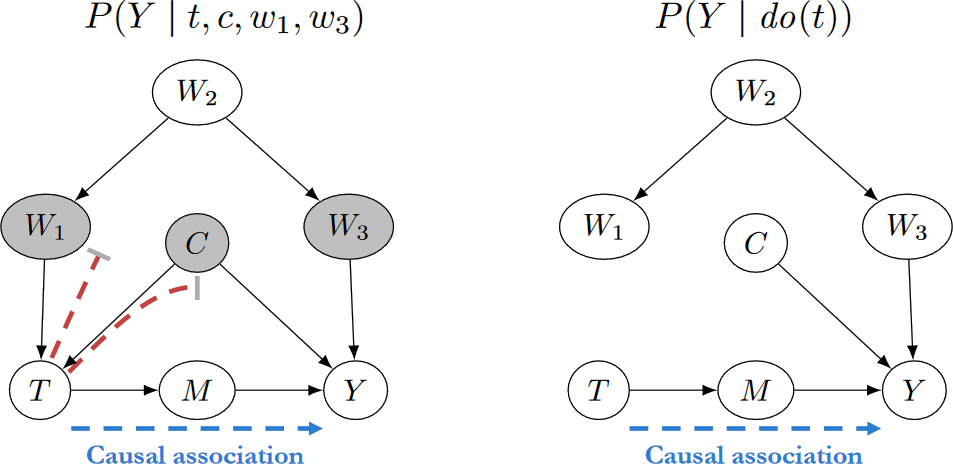
\includegraphics[width=.75\textwidth]{figures/ch3/22.backdoor.png}
    \caption{Backdoor paths blocked by conditioning on \( W \).}
    \vspace{-10px}
    \caption*{\scriptsize{Source: \cite{Neal_2020a}}}
    \label{fig:backdoor}
\end{figure}

\subsection{Structural Causal Models}
\label{sec:scm}

We need to be able to state that $A$ is a \textbf{cause} of $B$,
meaning that changing $A$ results in changes in $B$, but changing
$B$ does not result in changes in $A$.
This relationship is represented by the following
\textbf{structural equation}:
\begin{equation}
B := f(A) \label{eq:streq}
\end{equation}
where \( f \) is some function that maps $A$ to $B$.

However, the mapping between $A$ and $B$ in Equation \ref{eq:streq}
is \textbf{deterministic}. Ideally, we'd like to allow it to be
\textbf{probabilistic}, which allows room for some unknown
causes of $B$ that factor into this mapping.
We can then write the following:
\begin{equation}
B := f(A, U) \label{eq:strequn}
\end{equation}
where \( U \) is some unobserved random variable.
The graph for this simple structural equation is shown in Figure \ref{fig:struct_eq}.

\begin{figure}[H]
    \centering
    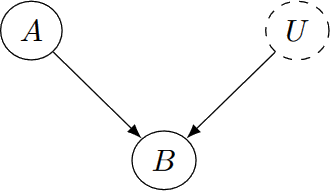
\includegraphics[width=.25\textwidth]{figures/ch3/23.struct_eq.png}
    \caption{Graph of \ref{eq:strequn}.
    The dashed node $U$ means that
    $U$ is unobserved.}
    \vspace{-10px}
    \caption*{\scriptsize{Source: \cite{Neal_2020a}}}
    \label{fig:struct_eq}
\end{figure}

While we have shown a single \textbf{structural equation}
in Equation \ref{eq:strequn}, there can be a large collection of
structural equations in a single model, commonly
labeled \( M \). For example, we write structural equations
for the causal model in Figure \ref{fig:scm} below:
\begin{equation}
M :
\begin{cases}
B := f_B(A, U_B) \\
C := f_C(A, B, U_C) \\
D := f_D(A, C, U_D)
\end{cases}
\label{eq:scm}
\end{equation}

\begin{figure}[H]
    \centering
    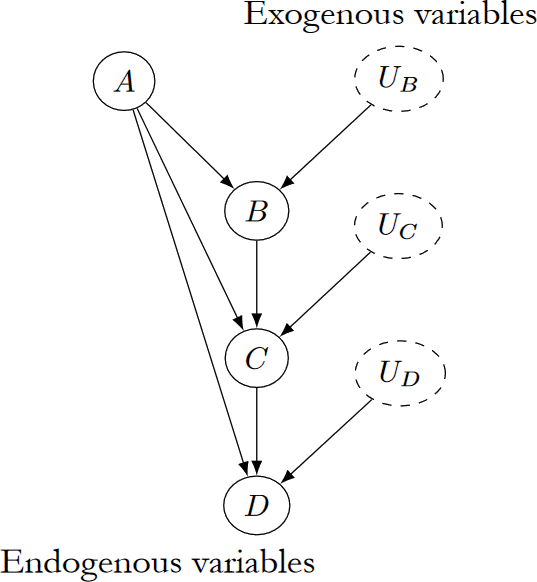
\includegraphics[width=.45\textwidth]{figures/ch3/24.scm.png}
    \caption{Graph of \ref{eq:scm}.}
    \vspace{-10px}
    \caption*{\scriptsize{Source: \cite{Neal_2020a}}}
    \label{fig:scm}
\end{figure}

The variables for which we write structural equations are known as
\textbf{endogenous variables}. These are the variables whose causal
mechanisms we are modeling.
In contrast, \textbf{exogenous variables} are variables that
do not have any parents in the causal graph.

\textbf{Structural Causal Model (SCM)}: a structural causal model
is a tuple consisting of the following sets:
\begin{enumerate}
    \item A set of endogenous variables \( V \)
    \item A set of exogenous variables \( U \)
    \item A set of functions \( f \), one to generate each
    endogenous variable as a function of other variables
\end{enumerate}